Die große freie Weglänge $\lambda$ ermöglicht den Elektronen, anders als den Ionen, erhebliche
Energie im elektrischen Feld zu gewinnen. Im elektrischen Feld erreichen Elektronen Energien von
einigen keV, sodass ihre deBroglie-Wellenlänge im Bereich der Atomdurchmessers liegt.
Quantenmechanische Interferenzeffekte führen zu starken Abhängigkeiten des Stoßquerschnitts $\sigma$
von der kinetischen Energie der Elektronen und damit auch der freien Weglänge $\lambda\approx
1/\sigma$.

% \begin{figure}[H]
% 	\centering
% 	
\includegraphics[width=0.5\textwidth]{dummy.jpg}
% \end{figure}

\begin{figure}[htbp]
	\begin{minipage}[b]{0.65\textwidth}
		\begin{figure}[H]
		\centering
		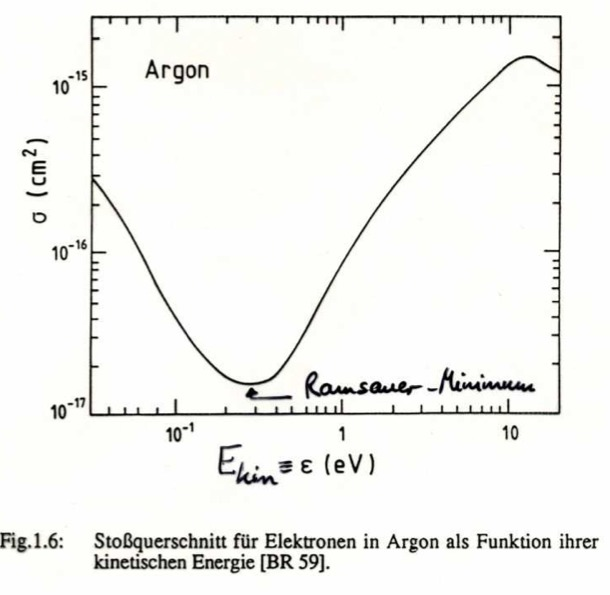
\includegraphics[width=\textwidth]{Fig-03-06.jpg}
		\end{figure}
	\end{minipage}
	\hspace{0.5cm}
	\begin{minipage}[b]{0.25\textwidth}
		\begin{figure}[H]
		\centering
		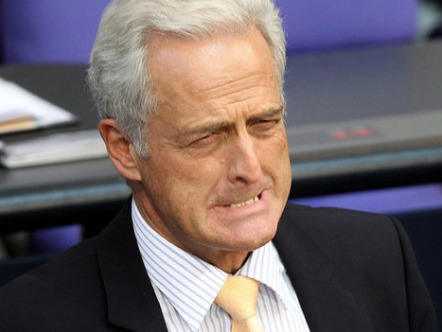
\includegraphics[width=\textwidth]{Fig-03-10a.jpg}
		\end{figure}
	\end{minipage}
	\caption{b}
	\label{rekristall} 
\end{figure}

Zur Herleitung einer Abschätzung der Driftgeschwindigkeit von Elektronen unter Einwirkung eines
elektrischen Feldes sei eine Gruppe von Elektronen mit thermischer Geschwindigkeit von

\[u=\sqrt{\frac{2E_{\text{kin}}}{m}}  \]

gegeben, die sich isotrop von einem Punkt $P$ fortbewegen:

\begin{figure}[H]
	\centering
	
\includegraphics[width=0.5\textwidth]{dummy.jpg}
\end{figure}

Unter Einwirkung eines elektrischen Feldes $\vec{E}$ werden aus den radialen Bahnen parabolische
Wege (Beschleunigung $\vec{b}=q\vec{E}/m$).

\begin{figure}[H]
	\centering
	
\includegraphics[width=0.5\textwidth]{dummy.jpg}
\end{figure}

$\delta_z$ ist die Verschiebung von $D+D_E$ entlang der z-Achse.
\\
Die Mittelung über alle cos$\,\Theta$ ergibt

\[ \langle \delta_z \rangle = \frac{1}{3}\cdot \frac{qE}{m}\cdot \langle t^2 \rangle \]

Für $\langle t^2 \rangle$ folgt durch die Mittelung der Laufzeiten über alle freien Weglängen $s$
und der thermicshen Elektronengeschwindigkeit $u$:

\[ \langle t^2 \rangle = \frac{\langle s^2 \rangle}{u^2} = \frac{2\lambda_e^2}{u^2} ,\]

wobei angenommen wurde, dass $\lambda_e$ unabhängig von $u$ ist (d.h. der Stoßquerschnitt $\sigma$
ist unabhängig von $u$). Damit ergibt sich als Driftgeschwindigkeit ($\langle t
\rangle=\lambda_e/u$):

\[v_D = \frac{\langle \delta_z \rangle}{\langle t\rangle} = \frac{2}{3}\cdot \frac{qE}{m}\cdot
\frac{\lambda_e}{u}\]

Zu berücksichtigen ist noch, dass die thermische Geschwindigkeit $u$ der Maxwell-Verteilung folgt.
Wird noch darüber gemittelt, so folgt

\[v_D\approx 0{,}92\cdot \frac{qE}{m}\cdot \frac{\lambda_e}{\sqrt{\langle
u^2\rangle}}~~~~~\text{mit}~~~~ \langle u^2\rangle = \frac{3kT}{m}\]

Zu beachten ist, dass $\lambda\sim \frac{1}{\text{Druck }p}$. Somit hängt $v_D$ explizit von der
reduzierten Feldstärke $E/p$ ab.
\\
Eine konstante Driftgeschwindigkeit erfordert, dass der Energiegewinn im $E-$Feld gleich
dem Energieverlust durch Stöße ist:

\[qE\cdot v_D\cdot \tau = \Delta(E_\text{kin})\cdot E_\text{kin}  \]

mit der Zeit $\tau$ zwischen zwei Stößen und dem Bruchteil der Energie $\Delta(E_\text{kin})$, die
beim Stoß auf das Gasatom übertragen wird. Es folgt

\[qE\cdot v_D = \frac{\Delta(E_\text{kin})\cdot E_\text{kin}}{\tau} =
\frac{\Delta(E_\text{kin})\cdot E_\text{kin}\cdot u}{\lambda_e}  \]

Für die konstante mittlere Driftgeschwindigkeit folgt dann weiterhin

\[qE\cdot v_D = \left\langle \frac{\Delta(E_\text{kin})\cdot E_\text{kin}}{\tau} \right\rangle =
\left\langle \frac{\Delta(E_\text{kin})\cdot E_\text{kin}\cdot u}{\lambda_e}\right\rangle \]

Um einige (quantitative) Aussagen über die Abhängigkeit der Driftgeschwindigkeit von der
elektrischen Feldstärke zu erhalten, sei im folgenden vereinfachend eine $\delta$-förmige
Geschwindigkeitsverteilung der für thermische Geschwindigkeit $u$ angenommen:

\[ E_\text{kin} = \frac{1}{2}\, m \cdot u^2 ~~~~~\Rightarrow ~~~~~ qE\cdot v_D\, \simeq\,
\frac{1}{2}\cdot \frac{\Delta(E_\text{kin})\cdot m\cdot u^3}{\lambda_e} , \]

sodass nach der Eliminierung von $u$ mittels

\[v_D = \frac{2}{3} \cdot \frac{qE}{m}\cdot \frac{\lambda_e}{u} \]

gilt:

\[v_D \approx \sqrt{\frac{2}{3}\sqrt{\frac{\Delta(E_\text{kin})}{3}}\cdot \frac{qE}{m}\cdot\lambda_e}
\]

Für die mittlere freie Weglänge $\lambda_e$ und den aufs Gasatom übertragenen Energiebruchteil
$\Delta(E_\text{kin})$ können als Näherung Potenzgesetze benutzt werden (vlg.
$\sigma-us-E$???-Diagramm und $\lambda_e\sim1/\sigma$):

\[\lambda_e(E_\text{kin})\sim E_\text{kin}^{-n}  \]
\[\Delta(E_\text{kin})\sim E_\text{kin}^{+m} \]

Aus der Eliminierung von $E_\text{kin}=\frac{1}{2}\,m\cdot u^2$ in $v_D = \frac{2}{3} \cdot
\frac{qE}{m}\cdot \frac{\lambda_e}{u}$ und $qE\cdot v_D\cdot \tau = \Delta(E_\text{kin})\cdot
E_\text{kin}\cdot \frac{u}{\lambda_e}$ ergibt sich

\[v_D \sim E ^{(m+1)/(m+2n+1)}  \]

Dies bedeutet für die Kurve $\sigma-us-E$??? von Argon:

\begin{itemize}
  \item $E$ liegt unterhalb des Ramsauer-Minimums: $n\approx -1$\\
  $\rightarrow (m+1)/(m+2n+1)\approx \frac{m+1}{m-1}$\\
  $\rightarrow$ für $m\gtrsim 1$ wird der Exponent groß, d.h. $v_D$ steigt schnell mit der
  Feldstärke $E$ an.
  \item $E$ liegt oberhalb des Ramsauer-Minimums: $n\approx +1$\\
  $\rightarrow (m+1)/(m+2n+1)\approx \frac{m+1}{m+3}$\\
  $\rightarrow$ für $m\gtrsim 1$ ist der Exponent $\ge1/2$, d.h. $v_D$ steigt nur noch geringfügig
  mit der Feldstärke $E$ an.
\end{itemize}

Im Falle molekularer Gase wie CO$_2$, CH$_4$ \ldots existieren Schwingungs- und Rotationsanregungen
bei recht geringen Energien. Diese Anregungen tragen stark zum gesamten Stoßquerschnitt bei, wobei
der übertragene Energieanteil $\Delta(E_\text{kin})$ sehr groß wird, um dann oberhalb der maximalen
Schwingungsenergie $E_\text{max}$ rasch abzunehmen.

\[\Delta(E_\text{kin}) \sim \frac{E_\text{max}}{E_\text{kin}}  \]

Für $E_\text{kin}>E_\text{max}$ ist $m\simeq 1$, d.h. $(m+1)/(m+2n+1)\approx 0$ und somit ist dort
$v_D=\,$const (z.B. für Ethen C$_2$H$4$).
\\
Im Falle, dass $\Delta(E_\text{kin})$ stärker als $1/E_\text{kin}$ abnimmt, wird $m<-1$, sodass
$v_D$ mit der elektrischen Feldstärke $E$ sogar wieder abnimmt (z.B. für CH$_4$). Daher können schon
kleine Verunreinigungen mit molekularen Gasen zu starken Veränderungen der Driftgeschwindigkeiten
führen.

\begin{figure}[H]
	\centering
	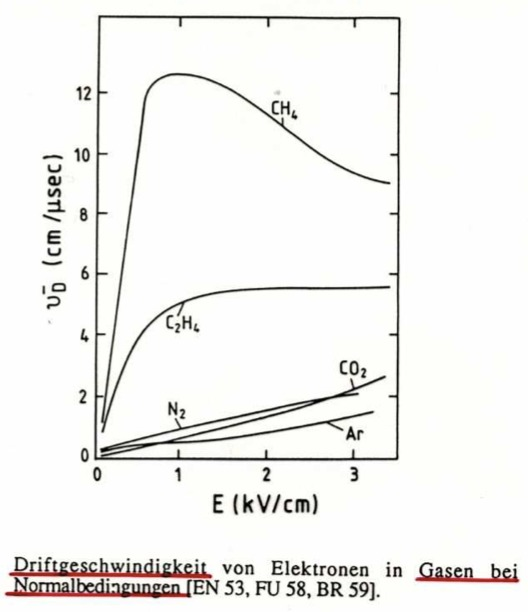
\includegraphics[width=0.5\textwidth]{Fig-03-07.jpg}
\end{figure}

\begin{figure}[H]
	\centering
	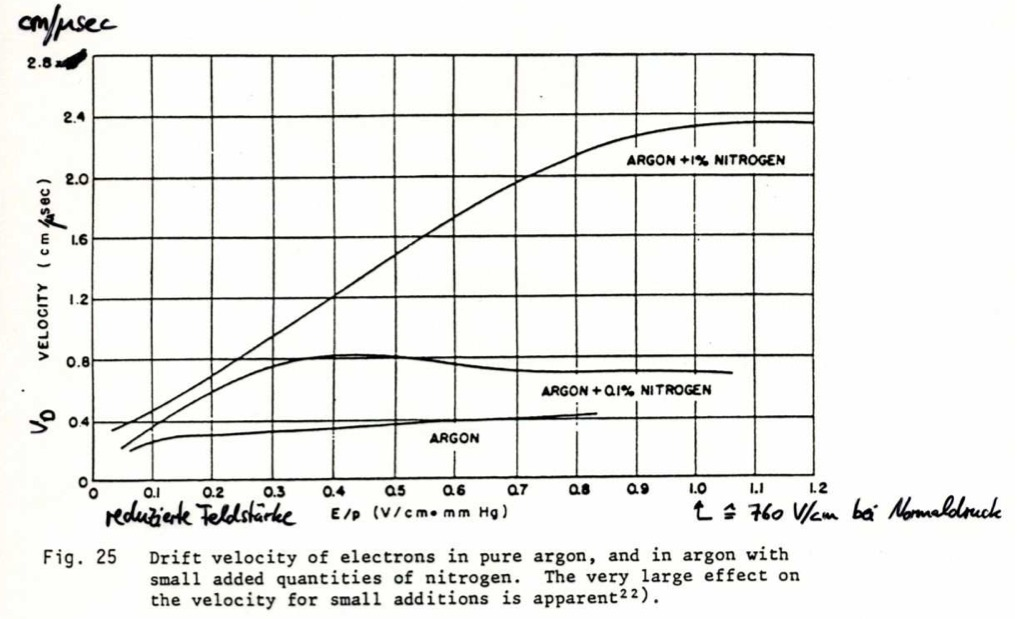
\includegraphics[width=0.7\textwidth]{Fig-03-08.jpg}
\end{figure}
